\documentclass[12pt,a4paper]{article}
\usepackage{amsmath}
\usepackage{amsfonts}
\usepackage{amssymb}
\usepackage{apacite}
\usepackage{graphicx}
\usepackage[top=2.5cm, bottom=2.5cm, left=2.5cm, right=2.5cm]{geometry}
\usepackage[toc,page]{appendix}
\usepackage{hyperref}
\usepackage{fancyref}
\usepackage[round]{natbib}
\usepackage{fancyhdr}
\usepackage{qtree}
\usepackage{booktabs}
\pagestyle{fancy}

\begin{document}

\title{Advanced Vision Assignment \# 1}
\author{Student Numbers s1107496 \& s1119520}

\maketitle

\section{Introduction}
In this assignment, we sought to track the motion of various balls over the course of a given video. To facilitate this, we were supplied with a representative background frame of the environment, as well as ground truth positions for each of the balls which could be used to evaluate our program.

\section{Methods}

\subsection{Frame processing pipeline}
To detect the balls within a frame, the frame went through a number of processing steps, which ultimately resulted in the detection of a number of connected components. These steps are described below.
\subsubsection{Background subtraction}
The function \texttt{background\_sub} was used to subtract the supplied background from the current frame, in order to isolate changed regions which potentially might be classified as balls. To achieve this, both the R channels of the RGB versions of the background and current frame and the S channels of the HSV versions of the background and current frame were isolated. For each of these channels, absolute differences between the established background and current frame values were calculated per-pixel, then thresholded using hand-optimized parameters. If a pixel significantly differed in either the R or S channels as per these thresholds, it was considered to be a non-background pixel. Finally, the resultant binary mask had the \texttt{bwmorph} ``\texttt{erode}" and ``\texttt{close}" functions applied to it, as well as \texttt{medfilt2}, in order to clean up stray pixels in the mask. 
\begin{figure}
	\centering
    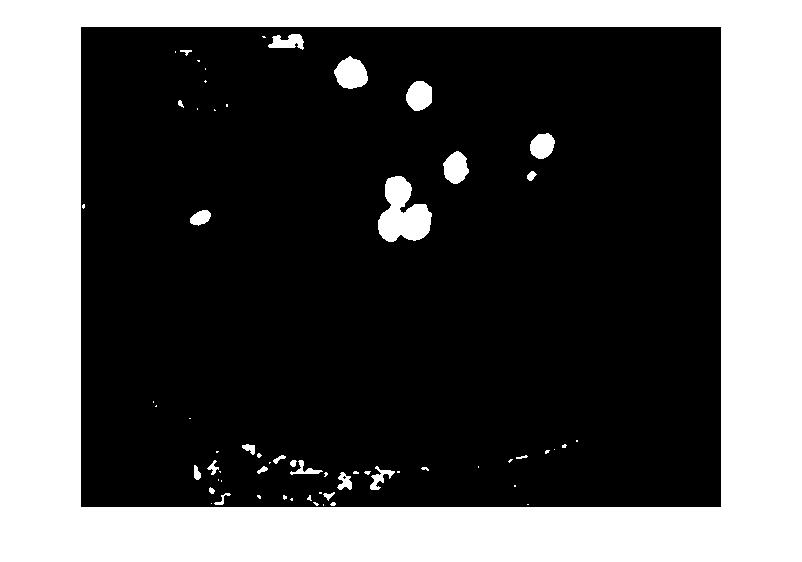
\includegraphics[width=140mm]{frame_35_imgs/background_sub.png}
    \caption{Resulting image after background substraction}
	\label{my-label0}
\end{figure}

\subsubsection{Separation of balls sharing a connected component}
In some instances, after background subtraction multiple balls may be located within the same connected component within our generated binary mask. This might result from a number of circumstances, including our background subtraction method being too sensitive, the motion blur of multiple balls overlapping, or one ball occluding another. In any case, we wish in these instances to separate the balls into multiple distinct connected components, for later use within our tracking system. 

To perform this step, we use the function \texttt{separate\_balls}, passing our background mask and the current frame. For each connected component within our background mask, we check to see whether its eccentricity is below a certain threshold. If the connected component has low eccentricity according to this threshold, we consider the connected component sufficiently ball-like such that we do not need to perform any separation. Following this, we apply the background mask to our current (RGB) frame, keying out the background and leaving only (potential) foreground objects. We also key out the previously found ball-like connected components. The resultant keyed frame is then passed to the \texttt{separate\_connected\_component} function.

In \texttt{separate\_connected\_component}, we convert the given masked image from RGB into HSV, then isolate the H and S channels. Following this, we apply the Scharr variant of the well-known Sobel edge-detection kernel in both the \texttt{x} and \texttt{y} directions to the respective channels, providing us derivatives with respect to hue and saturation both vertically and horizontally. In doing so, we are able to distinguish not only differently-colored balls from each other (by virtue of their differing hues and saturations) but also (under ideal circumstances) the background between balls from the balls themselves. We then threshold these derivatives to create further binary masks. Additionally, we isolate the background mask from the given image and apply the \texttt{bwmorph} ``\texttt{clean}" function. We then merge these five masks (including background mask) into a single mask by using the Matlab vector ``or" (\texttt{|}) operator. We finally apply various functions to improve the quality of the final mask, namely, \texttt{medfilt2} and \texttt{bwmporh} ``\texttt{erode}". We subsequently return this mask.

\begin{figure}
	\centering
    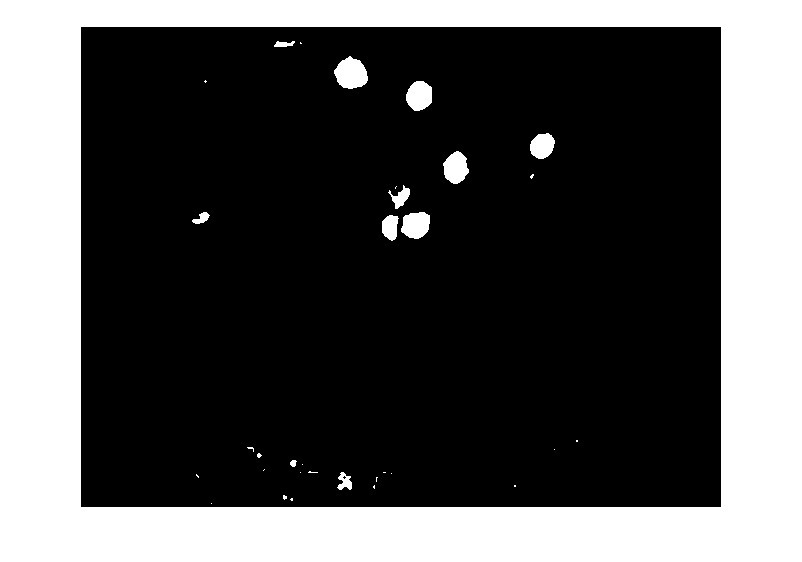
\includegraphics[width=140mm]{frame_35_imgs/separate_balls.png}
    \caption{Resulting image after separating connected components}
	\label{my-label01}
\end{figure}

\subsubsection{Final connected component extraction}
Finally, we extract all balls and their properties (in particular, centre position, area, diameter and pixel list of the connected component) in \texttt{extractForegroundObjects}. We apply 3 simple steps to remove components that are not likely to be balls - removing small or dark objects as well as only returning 10 largest components. Since we have area as part of the proporties for each of the connected component, we can then easily check if the area is larger than some predefined threshold (in our case, 50 pixels) and remove ones that are too small. We then remove objects that are dark and likely to be part of the background by converting all pixel values of the connected component to greyscale, finding the mean value (average luminocity) of all pixels in it and keeping only the ones that has average luminocty higher than a threshold.

Since, the total number of balls is known to be 10 we are sure that if we have more than 10 connected components then some of them are clearly not balls. Therefore, we only keep 10 largest objects assuming that noise objects are going to be smaller than any of the balls.

The result of \texttt{extractForegroundObjects} is the final list of all recognized balls in the frame.   

\begin{figure}
	\centering
    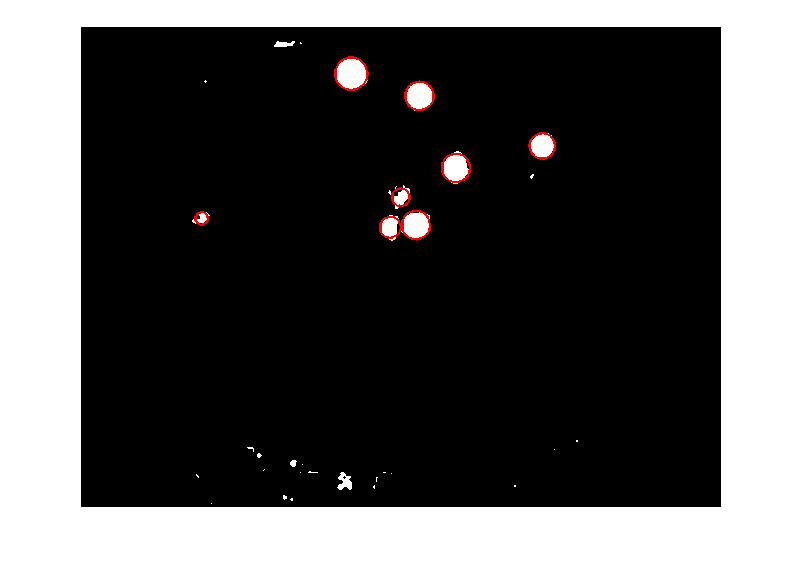
\includegraphics[width=140mm]{frame_35_imgs/extractForegroundObjects.png}
    \caption{Resulting image after extracting balls}
	\label{my-label02}
\end{figure} 

\subsection{Cross-frame object tracking}
Having isolated connected components, we then seek to match these to connected components (``objects") from previous frames within the function \texttt{update\_ball\_tracking}. Each object in the current frame is uniquely mapped to at most one object from previous frames. Matching between objects is performed by first calculating a number of respective properties given the object's connected component, as follows:
\begin{itemize}
\item the \texttt{x} and \texttt{y} coordinates of the connected components's centroid ($obj_x^{cur}$ and $obj_y^{cur}$, respectively),
\item the area of the connected component $obj_{a}^{cur}$,
\item the average hue of the pixels comprising the connected component $obj_{h}^{cur}$,
\item the average saturation of the pixels comprising the connected component $obj_{s}^{cur}$, and
\item the time at which the connected component was detected $obj_{t}^{cur}$ (i.e. the current time).
\end{itemize}
Further to this, the following properties are computed for each current object $obj^{cur}$ with respect to each potential match from a previous frame, $obj^{past}$, were $obj^{cur}$ to be matched with $obj^{past}$:
\begin{itemize}
\item the x-velocity $obj_{vx}^{cur}$ ($(obj_x^{cur} - obj_x^{past}) / (obj_t^{cur} - obj_t^{past})$) and y-velocity $obj_{vy}^{cur}$ ($(obj_y^{cur} - obj_y^{past}) / (obj_t^{cur} - obj_t^{past})$),
\item the overall object velocity $obj_{vm}^{cur}$ ($\sqrt{(obj_{vx}^{cur})^2 + (obj_{vy}^{cur})^2}$), and
\item the predicted x-position $obj_{px}^{past}$ ($obj_x^{past} + obj_{vx}^{past}$) and y-position $obj_{py}^{past}$ ($obj_y^{past} + obj_{vy}^{past}$) of the past object.
\end{itemize}
For each potential mapping between current and past objects, the mapping is immediately rejected if any of the following is true:
\begin{itemize}
\item the past object has already been matched to an object in the current frame,
\item the past object existed too long in the past, as determined by a time thresholding parameter, or
\item the calculated velocity of the current object if matched to the past object would exceed a set velocity thresholding parameter.
\end{itemize}
Otherwise, a cost is calculated for the mapping between objects by calculating a Euclidean distance between these properties in n-dimensional space, with each component approximately normalized to a value of 1 (e.g. $obj_{x}$ is divided by the width of the frame). Should this cost exceed a predetermined threshold, the mapping is discarded.

\begin{figure}
	\centering
    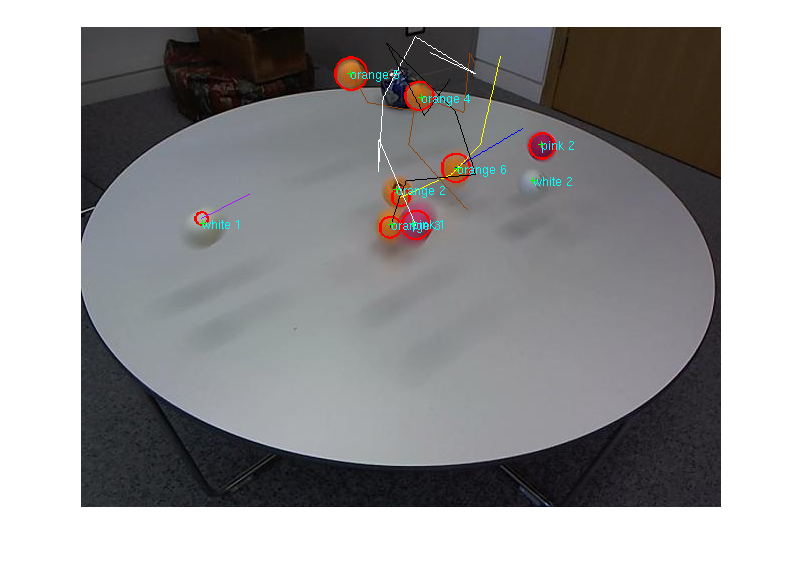
\includegraphics[width=140mm]{frame_35_imgs/update_ball_tracking.png}
    \caption{Resulting paths drawn on top of the frame}
	\label{my-label02}
\end{figure}

While minimizing the costs across all possible mappings constitutes an optimization problem, for the sake of simplicity we instead utilize a greedy ``first come, first served" approach whereby the first found connected component/object is paired with the best-matching past object not violating any of the above constraints, the second paired with any best-matching past object not including that matched to the first object, \textit{et cetera}. Finally, these mappings are used to determine \texttt{prev\_x} and \texttt{prev\_y} properties for the current objects, which are used when plotting object paths.

\section{Results}
Evaluation has been done in two steps. We evaluated our code's ability to recognize balls in each frame and the performance of the tracker. The results are explained in the next two subsections.

\subsection{Object recognition}
After we get the final list of objects recognized as balls, we then call our evaluation function \texttt{evaluate} that calculates the number of balls that were detected within 10 pixels of any ground truth, the mean distance between the ground truth and estimated centres for all such balls within the 10 pixel distance threshold, the number of false ball detections and the number of balls that were not detected. Results are presented in the following table:

\begin{table}[h]
\centering
\begin{tabular}{@{}cccc@{}}
\toprule
correct detections & incorrect detections & not detected & mean distance \\ \midrule
241                & 0                    & 32           & 2.5746        \\ \bottomrule
\end{tabular}
\caption{Ball detection results}
\label{my-label}
\end{table}

As we can see from the table above, we managed to correctly recognize 241 balls within 10 pixel distance with a mean distance just under 2.6 pixels. Our ball detector managed not to make any mistakes while recognizing the balls and, hence did not make any false detections.

Unfortunatelly, more than 30 balls could not be detected. Majority of these cases include either white ball being on top of white table or orange ball present over brown background where it is hard to capture it without recognizing any other additional noise or small ball on the ground where they are so small that are removed. Decreasing the minimum component size would not work since it includes lots of false detections. 

\begin{figure}
	\centering
    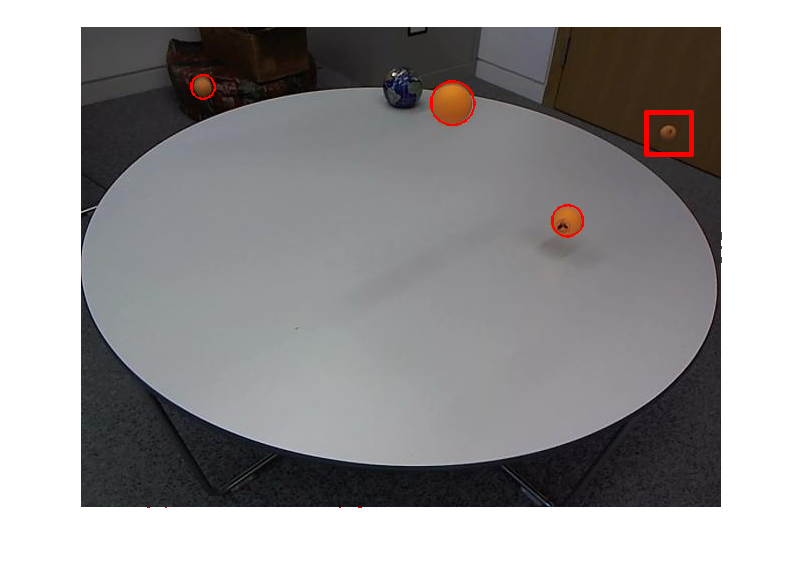
\includegraphics[width=140mm]{mistakes/frame_55_missed_ball.png}
    \caption{Brown looking orange ball over brown background could not be detected}
	\label{my-label06}
\end{figure} 

\subsection{Object tracking}
We have also evaluated our tracker. We found the number of correct and erroneous pairings as well as the percentage of ball detections that belong to trajectories with only 1 detection. We have also drawn an image of all ground truth trajectories on top of a background image \texttt{bgframe.jpg} as well as a separate image showing each of our predicted trajectories. By comparing these two images we made final tracking evaluation and calculated the number of tracked trajectories for each of the 10 balls. The results are shown in the table below:

\begin{table}[h]
\centering
\begin{tabular}{@{}cccc@{}}
\toprule
correct pairings & erroneous pairings & object detected once & ?? \\ \midrule
??                & ??                    & 3           & ??        \\ \bottomrule
\end{tabular}
\caption{Ball tracking results}
\label{my-label2}
\end{table}

\begin{figure}
	\centering
    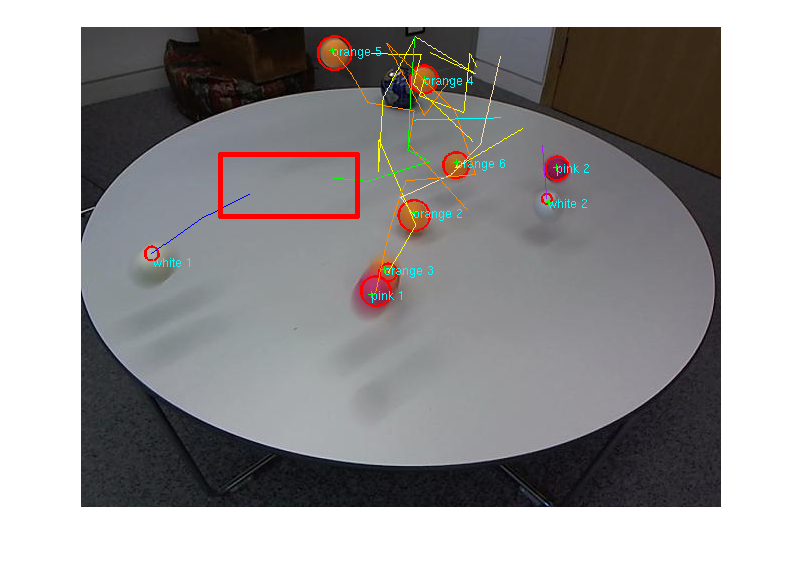
\includegraphics[width=140mm]{mistakes/tracking_breaks.png}
    \caption{Situation where our tracking breaks for white ball}
	\label{my-label07}
\end{figure} 

\begin{figure}
	\centering
    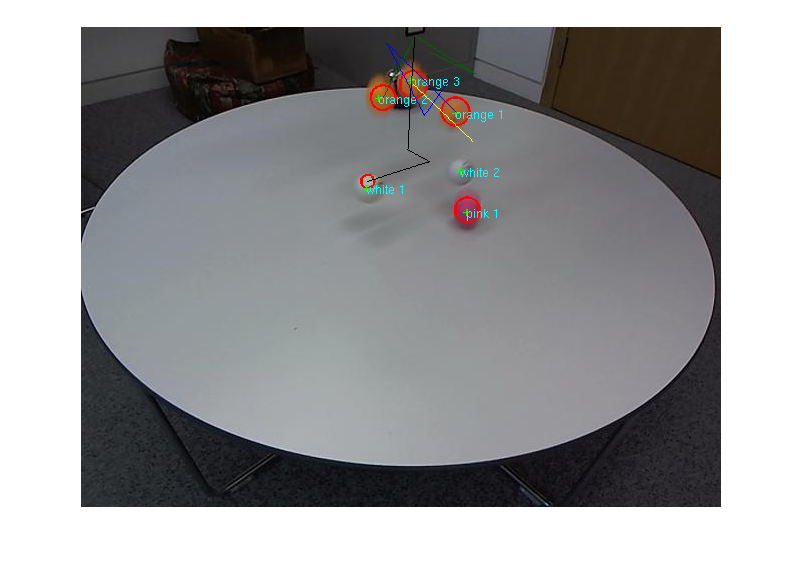
\includegraphics[width=140mm]{mistakes/frame_31_interobject_tracking_mismatches.png}
    \caption{???}
	\label{my-label08}
\end{figure} 

\begin{figure}
	\centering
    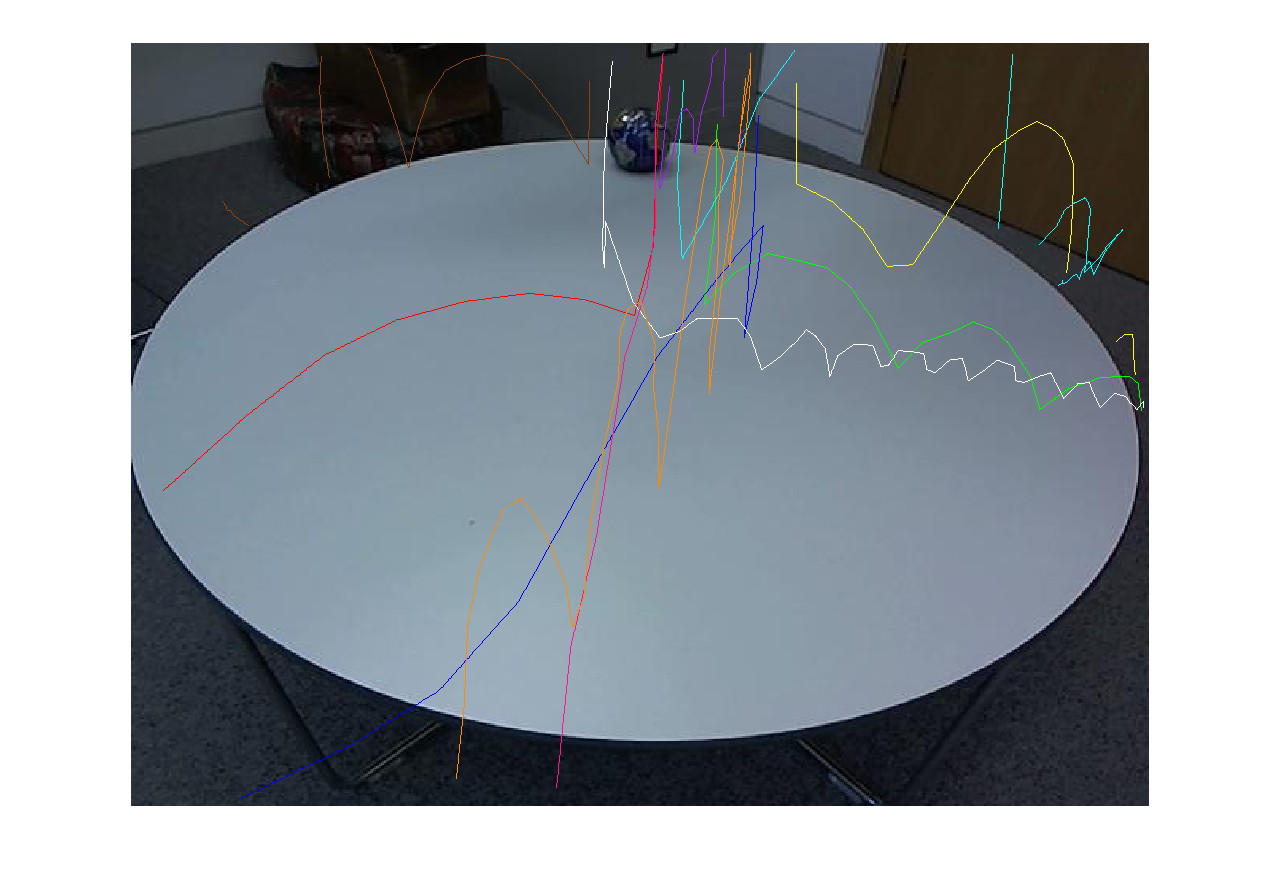
\includegraphics[width=140mm]{ground_truth_trajectories.png}
    \caption{Ground truth trajectories drawn on top of the background image}
	\label{my-label05}
\end{figure} 

\begin{figure}
	\centering
    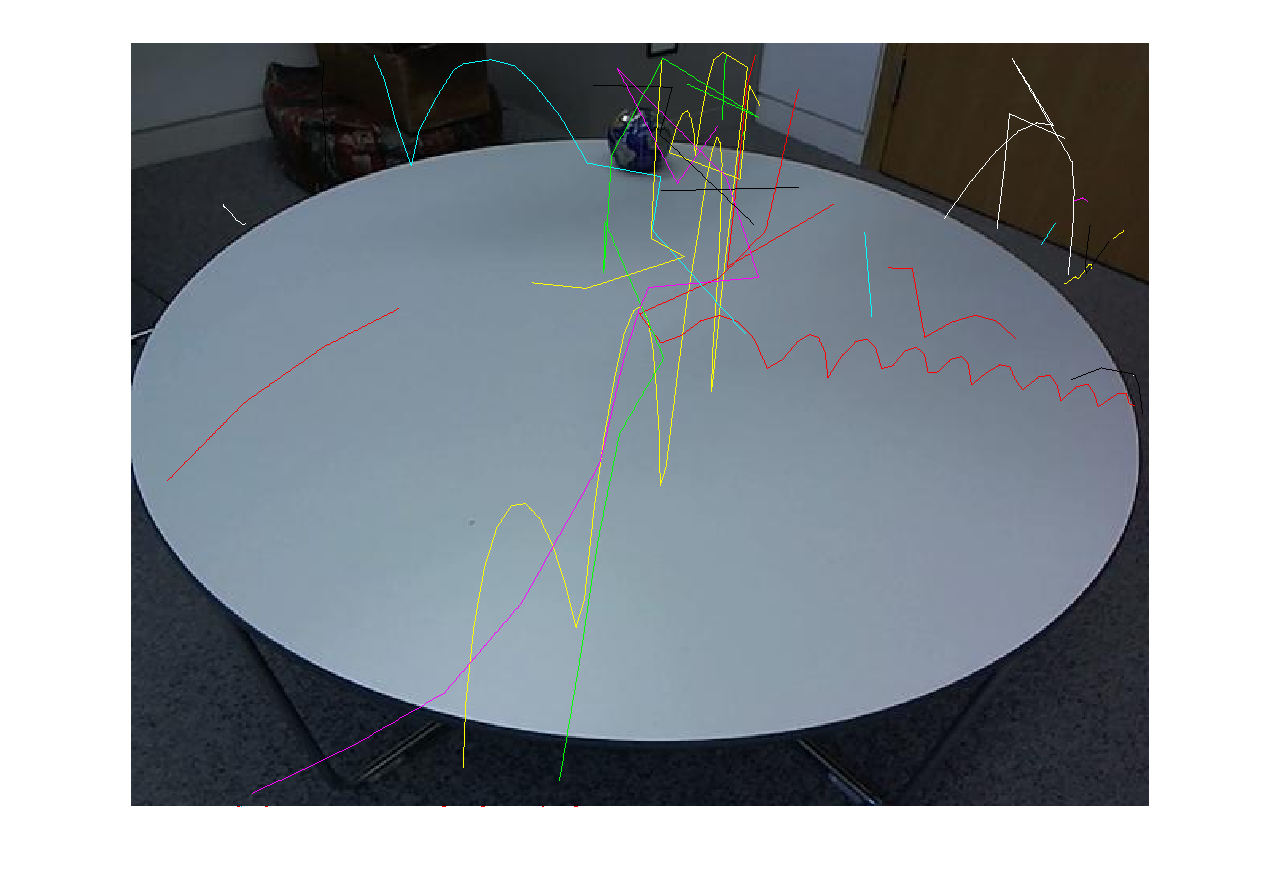
\includegraphics[width=140mm]{trajectories.png}
    \caption{Our predicted ball trajectories drawn on top of the background image}
	\label{my-label06}
\end{figure} 

\section{Discussion}
In this assignment we made the decision to eschew the condensity approach as presented in the lectures, as this was deemed needlessly complex for the requisite task. Although our tracking worked well in many situations, the implementation of condensity-based tracking may have better resolved issues with object tracking in the beginning of the video, as well as in later incidents in which our tracking/object linking system proved too brittle to handle tracking across more than two frames.

We also made the decision to use a non-probabilistic approach to background/foreground separation, especially having been given an example background frame. We did not feel this hindered our solution in any way, as our frame processing seemed quite robust, but it may have been useful to have explored a probabilistic approach in order to evaluate its advantages more concretely. 


\begin{appendices}
\section{Source code}

\subsection{drawpos.m}
\begin{verbatim}
load balls_loc.mat

num_balls = size(new_balls,2);
present = zeros(1, num_balls);
limits  = zeros(1, num_balls);
nextid  = ones(1, num_balls);
ball_name = {'white 1', 'white 2', 'pink 1', 'pink 2', 'orange 1', ...
 'orange 2', 'orange 3', 'orange 4', 'orange 5', 'orange 6'};
file_name='./set1/';
file_format='.jpg';

for i = 1:num_balls
	limits(i) = numel(new_balls(i).row_of_centers);
end

background = imread('bgframe.jpg');

tracked_balls = {};
tracked_balls{87} = {}; % 1 set for each frame

total_detections = zeros(1, 4);

for i = 25:87
	filename = [file_name sprintf('%08d', i) file_format];
	current_frame=imread(filename);
	clc
    substracted_frame = background_sub(current_frame, background);
    
    imshow(current_frame);
    hold on
       
    props = extractForegroundObjects(separate_balls(...
    substracted_frame, current_frame), current_frame);
    drawCentres(props);
    detections = evaluate(i, props);
    total_detections = total_detections + detections;
    
    tracked_balls = update_ball_tracking(props, current_frame, i,...
    tracked_balls);
    
    plot_paths(tracked_balls, i);
    
	for j = 1:num_balls
		limits(j) = numel(new_balls(j).row_of_centers);
		if nextid(j) <= limits(j)
			if new_balls(j).frame_numbers(nextid(j)) == i
				text(new_balls(j).row_of_centers(nextid(j)),...
				new_balls(j).col_of_centers(nextid(j)), ...
				ball_name{j}, 'Clipping', 'on', 'Color', 'cyan');
				plot(new_balls(j).row_of_centers(nextid(j)),...
				new_balls(j).col_of_centers(nextid(j)), 'g+');
				nextid(j) = nextid(j) + 1;
			end
        end
    end
	pause(1)
end

clc
imshow(background);
hold on
final_plot_paths(tracked_balls);

total_detections(1:3)
total_detections(4)/total_detections(1)
\end{verbatim}

\subsection{background\_sub.m}
\begin{verbatim}
function [ substracted_frame ] = background_sub(current_frame, background)

    % Get R values from RGB frame
    r_current_frame = current_frame(:, :, 1);
    r_background = background(:, :, 1);
    
    current_frame = rgb2hsv(current_frame);
    background = rgb2hsv(background);
    
    % Get S values from HSV frame
    s_current_frame = current_frame(:, :, 2);
    s_background = background(:, :, 2);
    
    y = size(current_frame, 1);
    x = size(current_frame, 2);
    
    % Create a mask for moving objects
    diff = ((abs(r_current_frame - r_background) > 25) |...
     (abs(s_current_frame - s_background)) > 0.25);
    
    substracted_frame = zeros(y, x);
    
    substracted_frame(diff) = 255;
    
    substracted_frame = bwmorph(substracted_frame, 'erode', 1);
    substracted_frame = bwmorph(substracted_frame, 'close', Inf);
    substracted_frame = medfilt2(substracted_frame);
end
\end{verbatim}

\subsection{draw\_line.m}
\begin{verbatim}
function [] = draw_line( x1, y1, x2, y2, color )

    % Adapted from personal code from a previous IVR assignment
	
    x_points = linspace(x1, x2, 50);  
    y_points = linspace(y1, y2, 50); 
    plot(x_points, y_points, 'Color', color);
    
end
\end{verbatim}

\subsection{draw\_truth.m}
\begin{verbatim}
load balls_loc.mat
background = imread('bgframe.jpg');
imshow(background)
hold on

COLORS = {'red', 'green', 'blue', 'yellow', 'cyan', 'white', ...
[255/255, 20/255, 147/255], [160/255, 32/255, 240/255], ...
[139/255, 69/255, 19/255], [1, 140/255, 0]};

num_balls = size(new_balls,2);

for i = 1:num_balls
    previous = new_balls(i).frame_numbers(1);
    for j = 2:size(new_balls(i).frame_numbers, 1)
        if previous + 1 == new_balls(i).frame_numbers(j)
            draw_line(new_balls(i).row_of_centers(j),...
            new_balls(i).col_of_centers(j),...
            new_balls(i).row_of_centers(j-1),...
            new_balls(i).col_of_centers(j-1), COLORS{i})
        end
        previous = new_balls(i).frame_numbers(j);
    end
end
\end{verbatim}

\subsection{drawCentres.m}
\begin{verbatim}
function drawCentres(props)
    centres = cat(1, props.Centroid);
    diameters = cat(1, props.EquivDiameter);
    % Draw centres of the objects
    for i = 1 : size(centres, 1)
        ang = 0:0.01:2*pi; 
        r = diameters(i)/2;
        xp = r*cos(ang);
        yp = r*sin(ang);
        plot(centres(i, 1)+xp, centres(i, 2)+yp, 'LineWidth', 2,...
        'Color', [1 0 0]); 
    end
end
\end{verbatim}

\subsection{evaluate.m}
\begin{verbatim}
function [detections] = evaluate(frame_id, props)
    load balls_loc.mat
    num_balls = size(new_balls,2);
    centers = cat(1, props.Centroid);
    
    correct_detections = 0;
    not_detected = 0;
    total_distance = 0;
    for i = 1:num_balls
        pos_index = find(new_balls(i).frame_numbers == frame_id);
        if isempty(pos_index)
            continue;
        end
        found_match = 0;
        for j = 1 : size(centers, 1)
            distance = norm(centers(j, :) -...
            [new_balls(i).row_of_centers(pos_index) ...
            new_balls(i).col_of_centers(pos_index)]);
            if distance <= 10
                total_distance = total_distance + distance;
                correct_detections = correct_detections + 1;
                found_match = 1;
                break;
            end
        end
        if ~found_match
            not_detected = not_detected + 1;
        end
    end
 
    incorrect_detections = size(centers, 1) - correct_detections;
    detections = [correct_detections incorrect_detections ...
    not_detected total_distance]
end
\end{verbatim}

\subsection{extractForegroundObjects.m}
\begin{verbatim}
function [ top_props ] = extractForegroundObjects(foreground, current_frame)
    MIN_AREA = 50;
    MIN_LUMINOSITY = 40;
    NUMBER_OF_BALLS = 10;
    
    current_frame_greyscale = rgb2gray(current_frame);
    
    % Find all the balls and their properties present in the frame
    props = regionprops(foreground, 'centroid', 'area',...
    'EquivDiameter', 'pixelList');
    
    % Remove small or dark objects (noise)
    rm = [];
    for i = 1 : length(props)
       % small
       if props(i).Area < MIN_AREA
          rm = [rm i];
          continue
       end
       
       % dark
       n_pixels = size(props(i).PixelList, 1);
       pixel_bw = zeros(n_pixels, 1);
       
       for p_i = 1 : n_pixels
           x = props(i).PixelList(p_i, 1);
           y = props(i).PixelList(p_i, 2);
           pixel_bw(p_i) = current_frame_greyscale(y, x);
       end
       
       if mean(pixel_bw) < MIN_LUMINOSITY
           rm = [rm i];
       end
       
    end
    
    props(rm) = [];
    
    % Find only 8-10 largest
    number_to_add = min(size(props, 1), NUMBER_OF_BALLS); 
    areas = cat(1, props.Area);
    if isempty(areas)
        top_props = props;
    else
        sorted_areas = sort(areas, 'descend');
        minimum_area = sorted_areas(number_to_add);
    
        top_props = props(1:number_to_add);
        k = 1;
        for i = 1 : size(props, 1)
            if props(i).Area >= minimum_area && k <= number_to_add
                top_props(k) = props(i);
                k = k + 1;
            end
        end
    end
end
\end{verbatim}

\subsection{final\_plot\_paths.m}
\begin{verbatim}
function [] = final_plot_paths( tracked_balls )

    % Adapted from personal code from a previous IVR assignment

    INITIAL_TIME = 25;
    FINAL_TIME = 87;

    for t = FINAL_TIME : -1 : INITIAL_TIME + 1
        num_objects = max(size(tracked_balls{t}));

        for obj_i = 1 : num_objects
            obj = tracked_balls{t}{obj_i};
            draw_line(obj.x, obj.y, obj.prev_x, obj.prev_y,...
            obj.color); 
        end
    end
end
\end{verbatim}

\subsection{plot\_paths.m}
\begin{verbatim}
function [] = plot_paths( tracked_balls, time )

    % Adapted from personal code from a previous IVR assignment

    INITIAL_TIME = 25;

    for t = time : -1 : INITIAL_TIME + 1
        num_objects = max(size(tracked_balls{t}));

        for obj_i = 1 : num_objects
            obj = tracked_balls{t}{obj_i};
            
            cur_object_count = max(size(tracked_balls{time}));
            for obj_j = 1 : cur_object_count
                cur_obj = tracked_balls{time}{obj_j};

                if strcmp(obj.id, cur_obj.id)
                    draw_line(obj.x, obj.y, obj.prev_x, obj.prev_y,...
                    obj.color); 
                    break
                end
            end
        end
    end
end
\end{verbatim}

\subsection{separate\_balls.m}
\begin{verbatim}
function [ background_mask ] = separate_balls( background_mask,...
current_frame )
    
    % Find all the objects and their properties present in the frame
    props = regionprops(background_mask, 'pixelList', ...
    'BoundingBox', 'Eccentricity', 'Centroid');
    % Separate balls from each connected component that seems to have
    % more than one ball in it
    allPixels = int16.empty;
    for i = 1 : size(props, 1)
        % First check if there might be more than one ball in the 
        % component
        if props(i).Eccentricity < 0.65
           continue
        end
        allPixels = [allPixels; props(i).PixelList];
    end
    
    % Create an image with visible components that might have more 
    % than one ball in it
    current_component = background_mask;
    current_component(background_mask ~= -1) = 0;
    for i = 1 : size(allPixels, 1)
        current_component(allPixels(i, 2), allPixels(i, 1)) = 255;
    end
    % Create a mask of these components
    mask = repmat(current_component, [1, 1, 3]);
    current_masked_image = current_frame;
    current_masked_image(~mask) = 0;
        
    % Separate balls in the components
    separated_component = separate_connected_component(current_masked_image);
    % Apply changes on the original substracted frame
    for i = 1 : size(allPixels, 1)
        background_mask(allPixels(i, 2), allPixels(i, 1)) =...
         separated_component(allPixels(i, 2), allPixels(i, 1));
    end
end

function [ balls ] = separate_connected_component(masked_image)
    hsv_image = rgb2hsv(masked_image);
    hue_values = hsv_image(:, :, 1);
    sat_values = hsv_image(:, :, 2);
    greyscale_image = rgb2gray(masked_image);
  
    % Scharr variant of Sobel kernel:
    x_kernel = [3 0 -3; 10 0 -10; 3 0 -3]; 
    y_kernel = [3 10 3; 0 0 0; -3 -10 -3]; 
    
    x_hue_convolved = conv2(hue_values, x_kernel, 'same');
    y_hue_convolved = conv2(hue_values, y_kernel, 'same');
    x_sat_convolved = conv2(sat_values, x_kernel, 'same'); 
    y_sat_convolved = conv2(sat_values, y_kernel, 'same');
    
    background = bwmorph(greyscale_image == 0, 'clean', 2);
    bool_x_hue_convolved = x_hue_convolved > 0.9;
    bool_y_hue_convolved = y_hue_convolved > 0.9;
    bool_x_sat_convolved = x_sat_convolved > 1;
    bool_y_sat_convolved = y_sat_convolved > 0.9;
    
    balls = bool_x_hue_convolved | ...
            bool_y_hue_convolved | ...
            bool_x_sat_convolved | ...
            bool_y_sat_convolved | ...
            background;
      
    balls = ~balls;
    balls = medfilt2(balls);
    balls = bwmorph(balls, 'erode', 1);  
end
\end{verbatim}

\subsection{update\_ball\_tracking.m}

\begin{verbatim}
function [ ball_history ] = update_ball_tracking( ...
 current_conn_comps, current_frame, time, ball_history )

    MIN_TIME = 25;
    FRAME_X = size(current_frame, 1);
    FRAME_Y = size(current_frame, 1);
    
    COLORS = {'red', 'green', 'blue', 'yellow', 'cyan', 'black',...
    'white', [255/255, 20/255, 147/255], [160/255, 32/255, 240/255],...
    [139/255, 69/255, 19/255], [1, 140/255, 0], [0, 100/255, 0],...
    [1, 222/255, 173/255]};
    
    % Distance function parameters - 
    % have tried to normalize these to ~1 
    A = 1 / (FRAME_X * FRAME_Y);  % Area
    X = 1 / FRAME_X;  % Centroid X
    Y = 1 / FRAME_Y;  % Centroid Y
    PREDICTED_X = 1 / FRAME_X; % Predicted centroid X (given prev. obj. vx)
    PREDICTED_Y = 1 / FRAME_Y; % Predicted centroid Y (given prev. obj. vy)
    T = 1;  % Time
    H = 1;  % Avg. hue
    S = 1;  % Avg. saturation
    VX = 1 / FRAME_X;  % X-velocity
    VY = 1 / FRAME_Y;  % Y-velocity
    VM = 1 / sqrt(FRAME_X * FRAME_Y);  % Velocity magnitude
    DIST_THRESH = 30;  % ! Will need some optimization !
    TIME_THRESH = 1;  % Only look N frames max back in time
    VM_THRESH = 0.25;  % Objects can only move this percentage of 
                       % the frame per time unit
    
    ball_history{time} = {};
    
    num_conn_comps = size(current_conn_comps, 1);  % should be no more than 10
    
    % not really sure what's up with this... 
    are_there_conn_comps = size(current_conn_comps, 2);  
    if ~are_there_conn_comps
        return
    end
    
    current_frame_hsv = rgb2hsv(current_frame);
    hues = current_frame_hsv(:, :, 1);
    sats = current_frame_hsv(:, :, 2);
    
    matched_obj_ids = {};
    n_matched_objs = 0;
    
    for cc_i = 1 : num_conn_comps
        cc = current_conn_comps(cc_i);
        cc_a = cc.Area;
        cc_x = cc.Centroid(1);
        cc_y = cc.Centroid(2);
        cc_t = time;
        
        n_pixels = size(cc.PixelList, 1);
        
        cc_hues = zeros(n_pixels);
        cc_sats = zeros(n_pixels);
        for p_i = 1 : n_pixels
            y = cc.PixelList(p_i, 1);
            x = cc.PixelList(p_i, 2);
            cc_hues(p_i) = hues(x, y);
            cc_sats(p_i) = sats(x, y);
        end
        cc_h = sum(sum(cc_hues)) / size(cc_hues, 1);  % sum of sums? why?
        cc_s = sum(sum(cc_sats)) / size(cc_sats, 1);
                
        best_match_id = 'NONE';
        best_match_score = -1;
        cc_vx = 0;
        cc_vy = 0;
        cc_vm = 0;
        cc_prev_x = 0;
        cc_prev_y = 0;
        % is -1 needed here? (error without)
        for t = max(MIN_TIME, (time - TIME_THRESH)) : (time - 1)  
            n_objects = max(size(ball_history{t}));
            for obj_i = 1 : n_objects
                obj = ball_history{t}{obj_i};
                
                % Enforce 1-to-1 mappings ... "first come, first served"
                already_matched = 0;
                for i = 1 : n_matched_objs
                    if strcmp(obj.id, matched_obj_ids{i})
                        already_matched = 1;
                    end
                end
                if already_matched == 1
                    continue
                end
                
                % Get proposed ball vector properties
                temp_cc_vx = (cc_x - obj.x) / (time - t);
                temp_cc_vy = (cc_y - obj.y) / (time - t);
                temp_cc_vm = sqrt(temp_cc_vx^2 + temp_cc_vy^2);
                
                if temp_cc_vm * VM > VM_THRESH
                    continue
                end
                
                % Comparison
                distance = sqrt(...
                    A * (cc_a - obj.a) ^ 2 + ...
                    X * (cc_x - obj.x + obj.vx) ^ 2 + ...
                    Y * (cc_y - obj.y) ^ 2 + ...
                    PREDICTED_X * (cc_x - (obj.x + obj.vx)) ^ 2 + ...
                    PREDICTED_Y * (cc_y - (obj.y + obj.vy)) ^ 2 + ...
                    T * (cc_t - obj.t) ^ 2 + ...
                    H * (cc_h - obj.h) ^ 2 + ...
                    S * (cc_s - obj.s) ^ 2 + ...
                    VX * (temp_cc_vx - obj.vx) ^ 2 + ...
                    VY * (temp_cc_vy - obj.vy) ^ 2 + ...
                    VM * (temp_cc_vm - obj.vm) ^ 2 ...
                );
            
                if distance > DIST_THRESH
                    continue
                end    
                
                if ((distance < best_match_score) ||...
                      strcmp(best_match_id, 'NONE'))
                    best_match_id = obj.id;
                    best_match_score = distance;
                    cc_vx = temp_cc_vx;
                    cc_vy = temp_cc_vy;
                    cc_vm = temp_cc_vm;
                    cc_prev_x = obj.x;
                    cc_prev_y = obj.y;
                    cc_color = obj.color;
                end
                
            end
        end
        
        if strcmp(best_match_id, 'NONE')
            best_match_id = strcat(num2str(time), '-', num2str(cc_i));
            cc_prev_x = cc_x;
            cc_prev_y = cc_y;
            color_i = randi(max(size(COLORS)));
            cc_color = COLORS{color_i};
        else
            % Record object ID as matched, so no other CCs can claim it:
            n_matched_objs = n_matched_objs + 1;
            matched_obj_ids{n_matched_objs} = best_match_id;
            
            % Commented out for now... with big enough emphasis on T comp.
            % or limit how far back in time matching can occur, hopefully
            % this will not be needed
            %for t = MIN_TIME : (time - 1)
            %    n_objects = size(ball_history{t});
            %    for obj_i = 1 : n_objects
            %        obj = ball_history{t}{obj_i};
            %        if strcmp(obj.id, best_match_id)
            %            % Get most recent location of object
            %            cc_prev_x = obj.x;
            %            cc_prev_y = obj.y;
            %        end
            %    end
            %end
        end
        
        ball_history{time}{cc_i} = struct( ...
            'id', best_match_id, ...
            'a', cc_a, ...
            'x', cc_x, ...
            'y', cc_y, ...
            't', cc_t, ...
            'h', cc_h, ...
            's', cc_s, ...
            'vx', cc_vx, ...
            'vy', cc_vy, ...
            'vm', cc_vm, ...
            'prev_x', cc_prev_x, ...
            'prev_y', cc_prev_y, ...
            'color', cc_color ...
        );
    
    end

end
\end{verbatim}

\end{appendices}

\end{document}
